\section{spazi metrici e topologia}
\index{spazio!metrico}

\begin{definition}[distanza indotta]
Se $d\colon X\times X \to \RR$ è una distanza su $X$
e $A \subset X$
allora restringendo $d$ ad $A \times A$ si ottiene ancora (ovviamente) una distanza.
Tale restrizione si chiama \emph{distanza indotta}
\mymargin{distanza indotta}%
\index{distanza!indotta}%
da $X$ su $A$.
Dunque se $A$ è un sottoinsieme di uno spazio metrico $(X,d)$ anche $A$ ha una struttura di spazio metrico.
\end{definition}

\begin{example}[sfera]
Se $X\subset \RR^n$ la distanza euclidea di $\RR^n$ induce
su $X$ una struttura di spazio metrico. Se $X$ non è un sottospazio vettoriale di $\RR^n$ abbiamo quindi esempi di spazi metrici che non sono spazi normati. Ad esempio
la \emph{sfera $n$-dimensionale}%
\mymargin{sfera $n$-dimensionale}%
\index{sfera}
\[
  \mathbb S^n = \ENCLOSE{\vec x \in \RR^{n+1}\colon \abs{\vec x} = 1}
\]
è uno spazio metrico con la distanza indotta da $\RR^n$.

Per $n=1$ si osserva che $\mathbb S^1$ è la circonferenza unitaria nel piano, 
per $n=2$ si ottiene l'usuale sfera unitaria immersa nello spazio tridimensionale.
\end{example}

\begin{definition}[palla]%
\label{def:palla}%
\mymark{*}%
Sia $(X,d)$ uno spazio metrico.
Per ogni $r>0$ e per ogni $x_0\in X$
definiamo la \emph{palla}%
\mymargin{palla}%
\index{palla} di raggio $r$ centrata in
$x_0$ come l'insieme
\[
  B_r(x_0) = \ENCLOSE{x\in X \colon d(x,x_0) < r}.
\]
\end{definition}

\begin{figure}
  \centering
  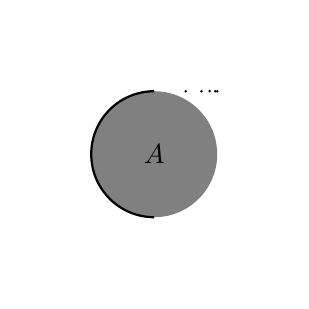
\begin{tikzpicture}[x=0.8cm,y=0.8cm]
    \draw[white] (2,-2) -- (2,2) -- (-2,2) -- (-2,-2) -- (2,-2);
    \fill[black!50] (0,0) circle (1);
    \draw[thick] (0,1) arc (90:270:1);
    \foreach \x in {0.5,0.75,0.88,0.97,1.0}
      \fill (\x,1) circle (0.5pt);
    \draw (0,0) node {$A$};
  \end{tikzpicture}
  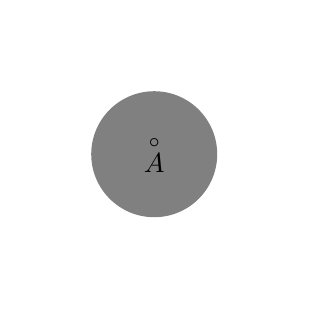
\begin{tikzpicture}[x=0.8cm,y=0.8cm]
    \draw[white] (2,-2) -- (2,2) -- (-2,2) -- (-2,-2) -- (2,-2);
    \fill[black!50] (0,0) circle (1);
    \draw (0,0) node {$\stackrel \circ A$};
  \end{tikzpicture}
  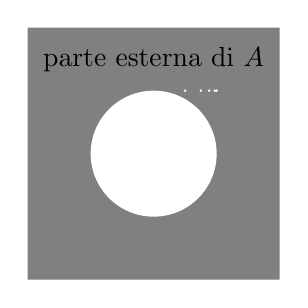
\begin{tikzpicture}[x=0.8cm,y=0.8cm]
    \fill[black!50] (2,-2) -- (2,2) -- (-2,2) -- (-2,-2) -- (2,-2);
    \foreach \x in {0.5,0.75,0.88,0.97,1.0}
      \fill[white] (\x,1) circle (0.5pt);
    \fill[white] (0,0) circle (1);
    \draw (0,1.5) node {parte esterna di $A$};
  \end{tikzpicture}
  \begin{tikzpicture}[x=0.8cm,y=0.8cm]
    \draw[white] (2,-2) -- (2,2) -- (-2,2) -- (-2,-2) -- (2,-2);
    \foreach \x in {0.5,0.75,0.88,0.97,1.0}
      \fill (\x,1) circle (0.5pt);
    \draw[thick] (1,0) arc (0:360:1);
    \draw (0,0) node {$\partial A$};
  \end{tikzpicture}
  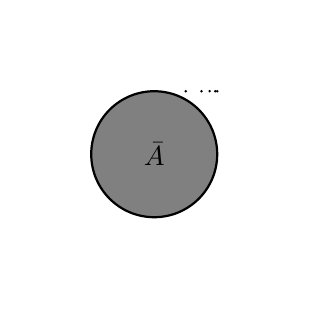
\begin{tikzpicture}[x=0.8cm,y=0.8cm]
    \draw[white] (2,-2) -- (2,2) -- (-2,2) -- (-2,-2) -- (2,-2);
    \foreach \x in {0.5,0.75,0.88,0.97,1.0}
      \fill (\x,1) circle (0.5pt);
    \fill[black!50] (0,0) circle (1);
    \draw[thick] (1,0) arc (0:360:1);
    \draw (0,0) node {$\bar A$};
  \end{tikzpicture}
  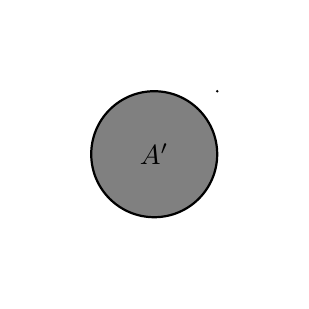
\begin{tikzpicture}[x=0.8cm,y=0.8cm]
    \draw[white] (2,-2) -- (2,2) -- (-2,2) -- (-2,-2) -- (2,-2);
    \fill (1,1) circle (0.5pt);
    \fill[black!50] (0,0) circle (1);
    \draw[thick] (1,0) arc (0:360:1);
    \draw (0,0) node {$A'$};
  \end{tikzpicture}
\caption{Un insieme $A$
e la sua parte interna $\stackrel \circ A$,
parte esterna, frontiera $\partial A$, chiusura $\bar A$ e punti di
accumulazione $A'$.}
\label{fig:}
\end{figure}


\begin{definition}[relazioni e proprietà topologiche]%
\mymark{*}%
\label{def:466342}%
Sia $(X,d)$ uno spazio metrico.
Un insieme $A\subset X$ si dirà essere un insieme
\emph{aperto}%
\mymargin{aperto}%
\index{aperto} in $X$ se per ogni $x\in A$ esiste $r>0$
tale che $B_r(x) \subset A$.
Un insieme $A\subset X$ si dirà essere un insieme 
\emph{chiuso}%
\mymargin{chiuso}%
\index{chiuso} in $X$ se il suo complementare $X\setminus A$ è aperto.

La famiglia di tutti gli insiemi aperti si chiama \emph{topologia}%
\mymargin{topologia}%
\index{topologia} dello spazio metrico $X$. 
Tutte le definizioni che seguono non dipendono dalla distanza $d$ ma solamente dalla topologia: 
basterà usare aperti qualunque al posto delle palle $B_r(x)$.

Se $A\subset X$ è un insieme qualunque
$x\in X$ è un punto qualunque diremo che:
\begin{enumerate}
\item
$x$ è \emph{punto interno}%
\mymargin{punto interno}%
\index{punto!interno} ad $A$ se esiste $r>0$ tale che $B_r(x) \subset A$;
chiameremo
\emph{parte interna}%
\mymargin{parte interna}%
\index{parte!interna}
di $A$ l'insieme dei punti interni di $A$
e la denoteremo con $\stackrel\circ A$;
\item
$A$ è un \emph{intorno}%
\mymargin{intorno}%
\index{intorno} di $x$ se $x$ è punto interno ad $A$
ovvero esiste $r>0$ tale che $B_r(x)\subset A$;
\item
$x$ è \emph{punto esterno}%
\mymargin{punto esterno}%
\index{punto!esterno} ad $A$ se è interno al complementare di $A$ ovvero esiste $r>0$ tale che $B_r(x) \cap A = \emptyset$;
chiameremo \emph{parte esterna}%
\mymargin{parte esterna}%
\index{parte!esterna} di $A$ l'insieme dei punti esterni ad $A$;
\item
$x$ è \emph{punto di frontiera}%
\mymargin{punto di frontiera}%
\index{punto!di frontiera} per $A$ se non è né interno né esterno ad $A$ ovvero per ogni $r>0$ l'insieme $B_r(x)$ contiene punti di $A$ e di $X\setminus A$;
chiameremo \emph{frontiera}%
\mymargin{frontiera}%
\index{frontiera} (o bordo) di $A$ l'insieme dei punti di frontiera che denoteremo con $\partial A$.
\item
$x$ è \emph{punto di aderenza}%
\mymargin{punto di aderenza}%
\index{punto!di aderenza} di $A$ se è interno o di frontiera ovvero se per ogni $r>0$ si ha $B_r(x) \cap A \neq \emptyset$;
chiameremo \emph{chiusura} di $A$ l'insieme dei punti di aderenza,
che denoteremo con $\bar A$;
\mymargin{chiusura}%
\index{chiusura}
\index{chiusura}
\item
$x$ è \emph{punto di accumulazione}%
\mymargin{punto di accumulazione}%
\index{punto!di accumulazione} di $A$ se
è punto di aderenza per $A \setminus \ENCLOSE{x}$ ovvero se
per ogni $r>0$ l'insieme $A \cap B_r(x)$ contiene punti diversi da $x$, chiameremo \emph{derivato}%
\mymargin{derivato}\index{derivato} di $A$ l'insieme dei punti di accumulazione (che si potrebbe denotare con $A'$);
\item
$x$ è \emph{punto isolato}%
\mymargin{punto isolato}\index{punto!isolato} di $A$ se è un punto di $A$ ma non di accumulazione per $A$ cioè se esiste $r>0$ per cui
$B_r(x) \cap A = \ENCLOSE{x}$.
\end{enumerate}
\end{definition}

\begin{theorem}[le palle sono aperte]
Sia $(X,d)$ uno spazio metrico, sia $x\in X$ e $r>0$. Allora la palla $B_r(x)$ è un insieme aperto in $X$.
\end{theorem}
%
\begin{proof}
Sia $y\in B_r(x)$: è sufficiente trovare $\rho>0$ tale che $B_\rho(y) \subset B_r(x)$. Prendendo $\rho = r-d(y,x)$ si osserva che $\rho >0 $ e, per la disuguaglianza triangolare,
dato $z \in B_\rho(y)$ si ha
\[
  d(z,x) \le d(z,y) + d(y,x) < \rho + d(y,x) = r
\]
da cui $B_\rho(y)\subset B_r(x)$ come volevamo dimostrare.
\end{proof}
